\newpage

\section{Appendice B: Intégrales Doubles}

\begin{definitionbox}[Intégrales Doubles]
Une \textbf{intégrale double} permet de calculer le volume sous une surface dans l'espace tridimensionnel, ou l'accumulation d'une quantité sur une région plane. Pour une fonction $f(x,y)$ définie sur un domaine $D \subset \mathbb{R}^2$, elle s'écrit :
$$ \iint_D f(x,y) \, dA = \iint_D f(x,y) \, dx\,dy $$
où $dA$ représente un élément d'aire infinitésimal.
\end{definitionbox}

\subsection{Construction pas à pas d'une intégrale double}

\begin{intuitionbox}[De l'intégrale simple à l'intégrale double]
L'objectif fondamental d'une intégrale double est d'étendre le concept d'accumulation (aire sous une courbe) à deux dimensions. Au lieu de sommer des rectangles de largeur $dx$ sous une courbe, on somme des \textbf{parallélépipèdes} de base $dx\,dy$ sous une surface. Le principe clé : \textbf{on intègre par étapes successives}, d'abord selon une variable en gardant l'autre fixe, puis selon la seconde variable.

Prenons l'exemple du calcul du volume sous la surface $f(x,y) = xy$ sur le rectangle $D = [0,1] \times [0,2]$.

\begin{enumerate}
    \item \textbf{Visualisation : Comprendre le domaine}
    \newline
    \textbf{Objectif :} Identifier la région d'intégration $D$ dans le plan $xy$.
    \newline
    \textbf{Notre cas :} $D$ est un rectangle avec $0 \le x \le 1$ et $0 \le y \le 2$. C'est le domaine le plus simple : les bornes sont constantes.
    \newline
    \textbf{Notation :} On écrira $\displaystyle\int_0^1 \int_0^2 xy \, dy\,dx$.

    \item \textbf{Première intégration : Fixer $x$, intégrer selon $y$}
    \newline
    \textbf{Objectif :} Pour chaque valeur fixée de $x$, calculer l'aire de la "tranche verticale" obtenue en variant $y$ de 0 à 2.
    \newline
    \textbf{Calcul :} On traite $x$ comme une constante et on intègre $xy$ par rapport à $y$ :
    $$ \int_0^2 xy \, dy = x \int_0^2 y \, dy = x \left[\frac{y^2}{2}\right]_0^2 = x \cdot \frac{4}{2} = 2x $$
    \textbf{Interprétation :} Le résultat $2x$ est une fonction de $x$ seulement. Elle représente l'aire de chaque tranche verticale à la position $x$.

    \item \textbf{Seconde intégration : Sommer toutes les tranches}
    \newline
    \textbf{Objectif :} Additionner les contributions de toutes les tranches verticales en intégrant selon $x$ de 0 à 1.
    \newline
    \textbf{Calcul :}
    $$ \int_0^1 2x \, dx = 2 \int_0^1 x \, dx = 2 \left[\frac{x^2}{2}\right]_0^1 = 2 \cdot \frac{1}{2} = 1 $$
    \textbf{Résultat final :} Le volume sous la surface $f(x,y)=xy$ sur $D$ est $\mathbf{1}$.

    \item \textbf{L'ordre d'intégration peut être inversé}
    \newline
    On aurait pu intégrer d'abord selon $x$, puis selon $y$ :
    $$ \int_0^2 \int_0^1 xy \, dx\,dy = \int_0^2 \left[\frac{x^2y}{2}\right]_0^1 dy = \int_0^2 \frac{y}{2} \, dy = \left[\frac{y^2}{4}\right]_0^2 = 1 $$
    \textbf{Principe de Fubini :} Pour les domaines rectangulaires avec fonctions continues, l'ordre d'intégration n'affecte pas le résultat, mais un ordre peut être plus simple que l'autre selon la fonction.

    \item \textbf{Le schéma général : Domaines non rectangulaires}
    \newline
    Lorsque $D$ n'est pas un rectangle, les bornes de l'intégrale intérieure dépendent de la variable extérieure.
    \newline
    \textbf{Exemple :} Si $D$ est délimité par $0 \le x \le 1$ et $0 \le y \le x^2$, on écrit :
    $$ \iint_D f(x,y) \, dA = \int_0^1 \int_0^{x^2} f(x,y) \, dy\,dx $$
    Les bornes $0$ et $x^2$ pour $y$ changent avec $x$, définissant ainsi la forme courbe de $D$.
\end{enumerate}
\end{intuitionbox}

\subsection{Intuition géométrique de l'intégrale double}

\begin{intuitionbox}[Interpréter l'intégrale double comme un volume]
Une intégrale simple $\int_a^b f(x) \, dx$ calcule l'aire sous une courbe. Une intégrale double $\iint_D f(x,y) \, dA$ calcule le \textbf{volume sous une surface} $z=f(x,y)$ au-dessus d'un domaine plan $D$.

\textbf{Cas particulier : Aire d'une région plane}
\newline
Si $f(x,y) = 1$ partout sur $D$, alors :
$$ \iint_D 1 \, dA = \text{Aire}(D) $$
L'intégrale double de la fonction constante 1 donne simplement l'aire du domaine.

\tcblower
\centering
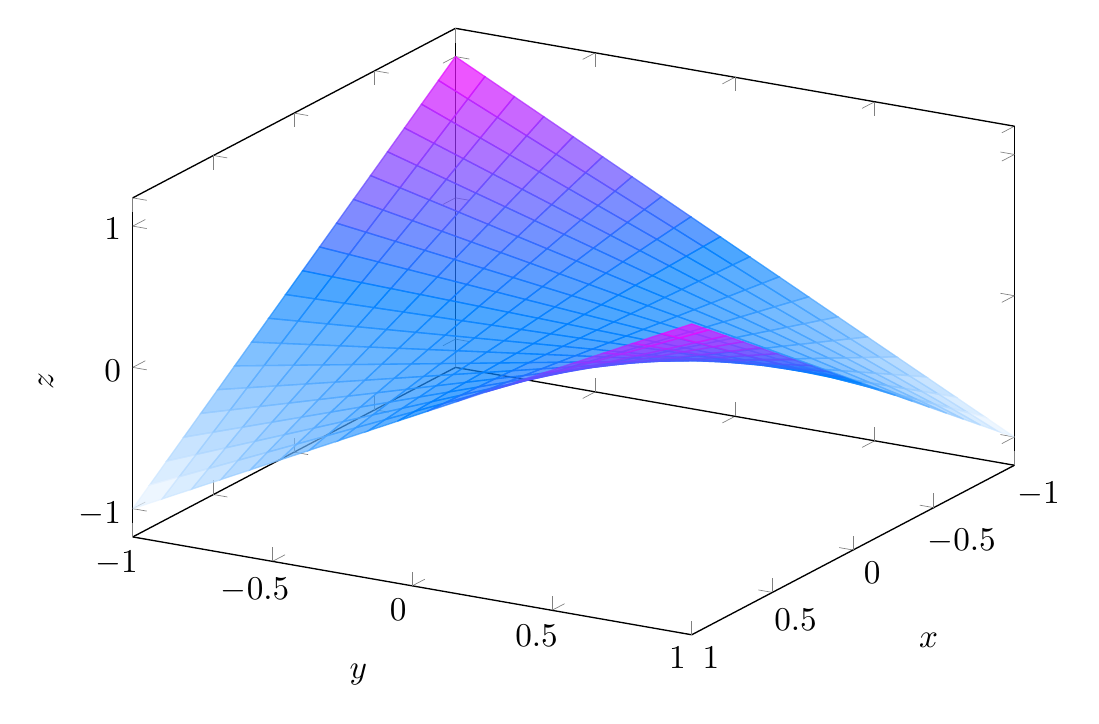
\begin{tikzpicture}[scale=1.2]
    \begin{axis}[
        view={120}{30},
        xlabel={$x$},
        ylabel={$y$},
        zlabel={$z$},
        domain=-1:1,
        y domain=-1:1,
        samples=20,
        height=8cm,
        width=0.9\linewidth,
        colormap/cool,
    ]
    
    \addplot3[
        surf,
        shader=flat,
        opacity=0.7,
    ] {x*y};
    
    \end{axis}
\end{tikzpicture}
\par\small\textit{Surface $z=xy$ au-dessus d'un domaine carré. Le volume sous cette surface est donné par l'intégrale double.}
\end{intuitionbox}


\subsection{Le Théorème de Fubini}

\begin{theorembox}[Théorème de Fubini]
Si $f(x,y)$ est continue sur le rectangle $R = [a,b] \times [c,d]$, alors :
$$ \iint_R f(x,y) \, dA = \int_a^b \int_c^d f(x,y) \, dy\,dx = \int_c^d \int_a^b f(x,y) \, dx\,dy $$
L'intégrale double peut être calculée comme deux intégrales simples itérées, et l'ordre d'intégration peut être inversé.
\end{theorembox}

\begin{intuitionbox}[Choisir le bon ordre d'intégration]
Bien que le théorème de Fubini garantisse que les deux ordres donnent le même résultat, l'un peut être beaucoup plus simple à calculer que l'autre.

\textbf{Exemple : $\displaystyle\iint_D e^{y^2} \, dA$ où $D = \{(x,y) : 0 \le x \le 1, \, x \le y \le 1\}$}

\textbf{Ordre 1 : Intégrer d'abord selon $x$, puis selon $y$}
\newline
Il faut reformuler les bornes : pour $0 \le y \le 1$, on a $0 \le x \le y$.
$$ \int_0^1 \int_0^y e^{y^2} \, dx\,dy = \int_0^1 e^{y^2} [x]_0^y \, dy = \int_0^1 y e^{y^2} \, dy $$
Par substitution $u=y^2$, $du=2y\,dy$ :
$$ = \frac{1}{2} \int_0^1 e^u \, du = \frac{1}{2}[e^u]_0^1 = \frac{e-1}{2} $$

\textbf{Ordre 2 : Intégrer d'abord selon $y$, puis selon $x$}
$$ \int_0^1 \int_x^1 e^{y^2} \, dy\,dx $$
L'intégrale $\int e^{y^2} \, dy$ n'a pas de forme close élémentaire ! Cet ordre est impraticable.

\textbf{Leçon :} Toujours examiner la fonction et le domaine avant de choisir l'ordre d'intégration.

\end{intuitionbox}

\subsection{Changement de l'ordre d'intégration : Exemple simple}

\begin{examplebox}[Exemple concret : Triangle]
Calculons l'intégrale : $$\int_0^1 \int_0^x y \, dy \, dx$$

\textbf{Région d'intégration initiale :}
\begin{itemize}
    \item $x$ varie de 0 à 1
    \item Pour chaque $x$ fixé, $y$ varie de 0 à $x$
\end{itemize}

C'est un \textbf{triangle} : $D = \{(x,y) : 0 \le x \le 1 \text{ et } 0 \le y \le x\}$

\tcblower

\textbf{Méthode 1 : Ordre initial (on intègre d'abord en $y$)}

\begin{align*}
\int_0^1 \left(\int_0^x y \, dy\right) dx &= \int_0^1 \left[\frac{y^2}{2}\right]_0^x dx \\
&= \int_0^1 \frac{x^2}{2} \, dx \\
&= \left[\frac{x^3}{6}\right]_0^1 \\
&= \frac{1}{6}
\end{align*}

\tcblower

\textbf{Méthode 2 : Changement de l'ordre (on intègre d'abord en $x$)}

\textit{L'astuce :} Redécrire la même région en fixant $y$ d'abord !

Dans le triangle, si je fixe $y$ :
\begin{itemize}
    \item $y$ varie de 0 à 1 (minimum et maximum de $y$ dans le triangle)
    \item Pour chaque $y$ fixé, $x$ varie de $y$ à 1 (car $x \ge y$ dans notre région)
\end{itemize}

\textbf{Nouvelles bornes :}
$$ \int_0^1 \int_y^1 y \, dx \, dy $$

\textbf{Calcul :}
\begin{align*}
\int_0^1 \left(\int_y^1 y \, dx\right) dy &= \int_0^1 y[x]_y^1 \, dy \\
&= \int_0^1 y(1-y) \, dy \\
&= \int_0^1 (y - y^2) \, dy \\
&= \left[\frac{y^2}{2} - \frac{y^3}{3}\right]_0^1 \\
&= \frac{1}{2} - \frac{1}{3} \\
&= \frac{1}{6} \quad \checkmark
\end{align*}
\end{examplebox}